\clearpage{\pagestyle{empty}\cleardoublepage}
\chapter{Introduzione al fotovoltaico}
%
Per \emph{impianto fovoltaico} si intende un qualunque 
impianto di produzione di energia elettrica che sfrutti, ai fini 
di produzione della stessa, l'\emph{effetto fotovoltaico}.
%
Ne esistono due grandi tipologie: impianti \emph{a isola} (o \emph{stand alone}), 
e impianti \emph{grid connected}, ovvero connessi alla rete nazionale in 
corrente alternata.
%
Oggetto di questa tesi saranno solo questi ultimi, in quanto sono gli unici
di cui abbia senso monitorare e quantificare la produzione energetica; gli impianti 
a isola, infatti, non sono generalmente utilizzati per la produzione di grandi
quantit\`a d'energia, piuttosto trovano applicazione laddove \`e necessario
rendere un sistema elettricamente \emph{autosufficiente}, p.es. per la 
ricarica di dispositivi alimentati a batteria.
%

%
Iniziamo la panoramica sugli impianti fotovoltaici partendo dal fenomeno
che sta alla base del loro funzionamento: l'effetto fotovoltaico.
%

%
\section{L'effetto fotovoltaico}
L'\emph{effetto fotovoltaico} consiste nel passaggio di elettroni 
dalla \emph{banda di valenza} alla \emph{banda di conduzione} di 
un materiale, a causa dell'assorbimento di \emph{fotoni}. 
%
Tale fenomeno viene sfruttato dai \emph{moduli (o celle) fotovoltaici}, 
come mostrato in figura \ref{effetto-fv} allo scopo di trasformare 
l'energia insita nella radiazione luminosa in energia elettrica.
%
\begin{figure}[!h]
\centering
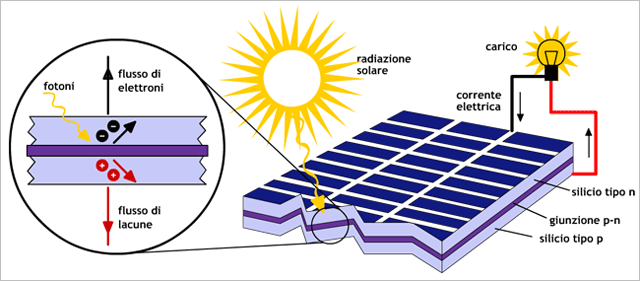
\includegraphics[width=350pt]{img/effetto-fovoltaico.png}
\caption{Effetto fotovoltaico}
\label{effetto-fv}
\end{figure}
%

%
\section{Architettura degli impianti grid-connected}
Gli impianti fotovoltaici grid connected, detti anche \emph{campi fotovoltaici}, 
sono costituiti da un insieme di dispositivi \emph{in cascata}, come mostrato in 
figura \ref{impiantogridconnect}: \emph{a monte} di tutto si trovano i \emph{moduli 
fotovoltaici}, ovvero i dispositivi che, sfruttando l'effetto fotovoltaico, 
producono energia elettrica. \emph{A valle} di questi, troviamo gli \emph{inverter}, 
macchinari il cui compito \`e quello di trasformare l'energia prodotta dai moduli 
in una forma tale che possa essere ceduta alla rete di distribuzione. Infine, tra 
gli inverter e la rete, il GSE provvede all'installazione di un \emph{contatore 
bidirezionale}, il cui scopo \`e quello di quantificare la produzione dell'impianto.
%% un impianto si caratterizza per la quantita` di energia di picco
\begin{figure}[!h]
\centering
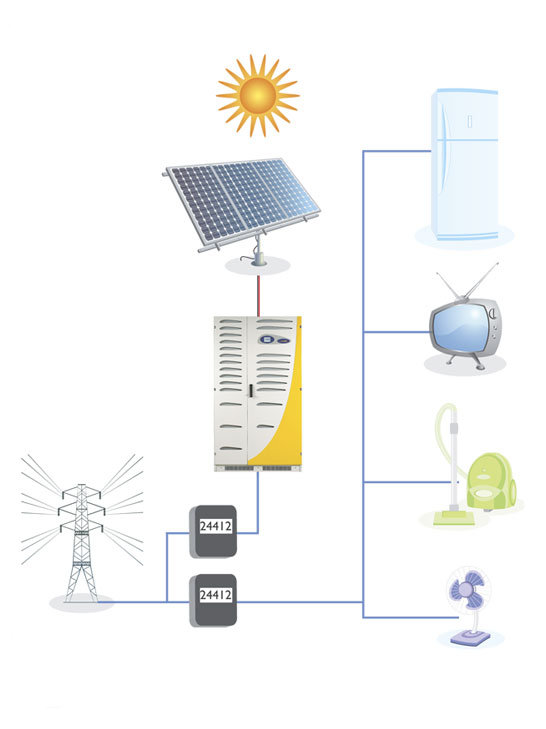
\includegraphics[width=350pt]{img/impianto-grid-connect.jpg}
\caption{Schema di impianto grid-connected con scambio sul posto}
\label{impiantogridconnect}
\end{figure}
%

%
Come gi\`a anticipato, gli impianti grid-connected immettono direttamente in rete 
l'energia prodotta. Per questo tipo di impianti, il GSE prevede uno schema di compensazione 
noto come \emph{scambio sul posto}\cite{scambioposto}, secondo cui l'energia immessa 
in rete pu\`o essere prelevata successivamente per i propri consumi.
%

%
\subsection{I moduli fotovoltaici}
I moduli fotovoltaici sono gli elementi produttivi di un impianto. 
Si tratta di dispositivi costituiti da \emph{celle} di materiale 
\emph{semiconduttore}, caratterizzato quindi da un \emph{band gap} 
di dimensioni tali per cui 
%
\begin{itemize}
\item a seguito dell'apporto energetico fornito dalla radiazione luminosa, 
      gli elettroni riescono a \emph{saltare} dalla banda di valenza a 
      quella di conduzione\footnote{ci\`o non sarebbe possibile in un \emph{isolante}}
%
\item gli elettroni che effettuano il \emph{salto} nella banda di conduzione 
      non vengono neutralizzati
      \footnote{come, invece, avverrebbe in un \emph{conduttore}}
\end{itemize}
%
La presenza di \emph{portatori di carica} nella banda di conduzione 
fa si che il modulo fotovoltaico, una volta connesso ad un conduttore 
esterno, si comporti come un \emph{generatore di corrente}\cite{bellini09}.
%
\begin{figure}[!h]
\centering
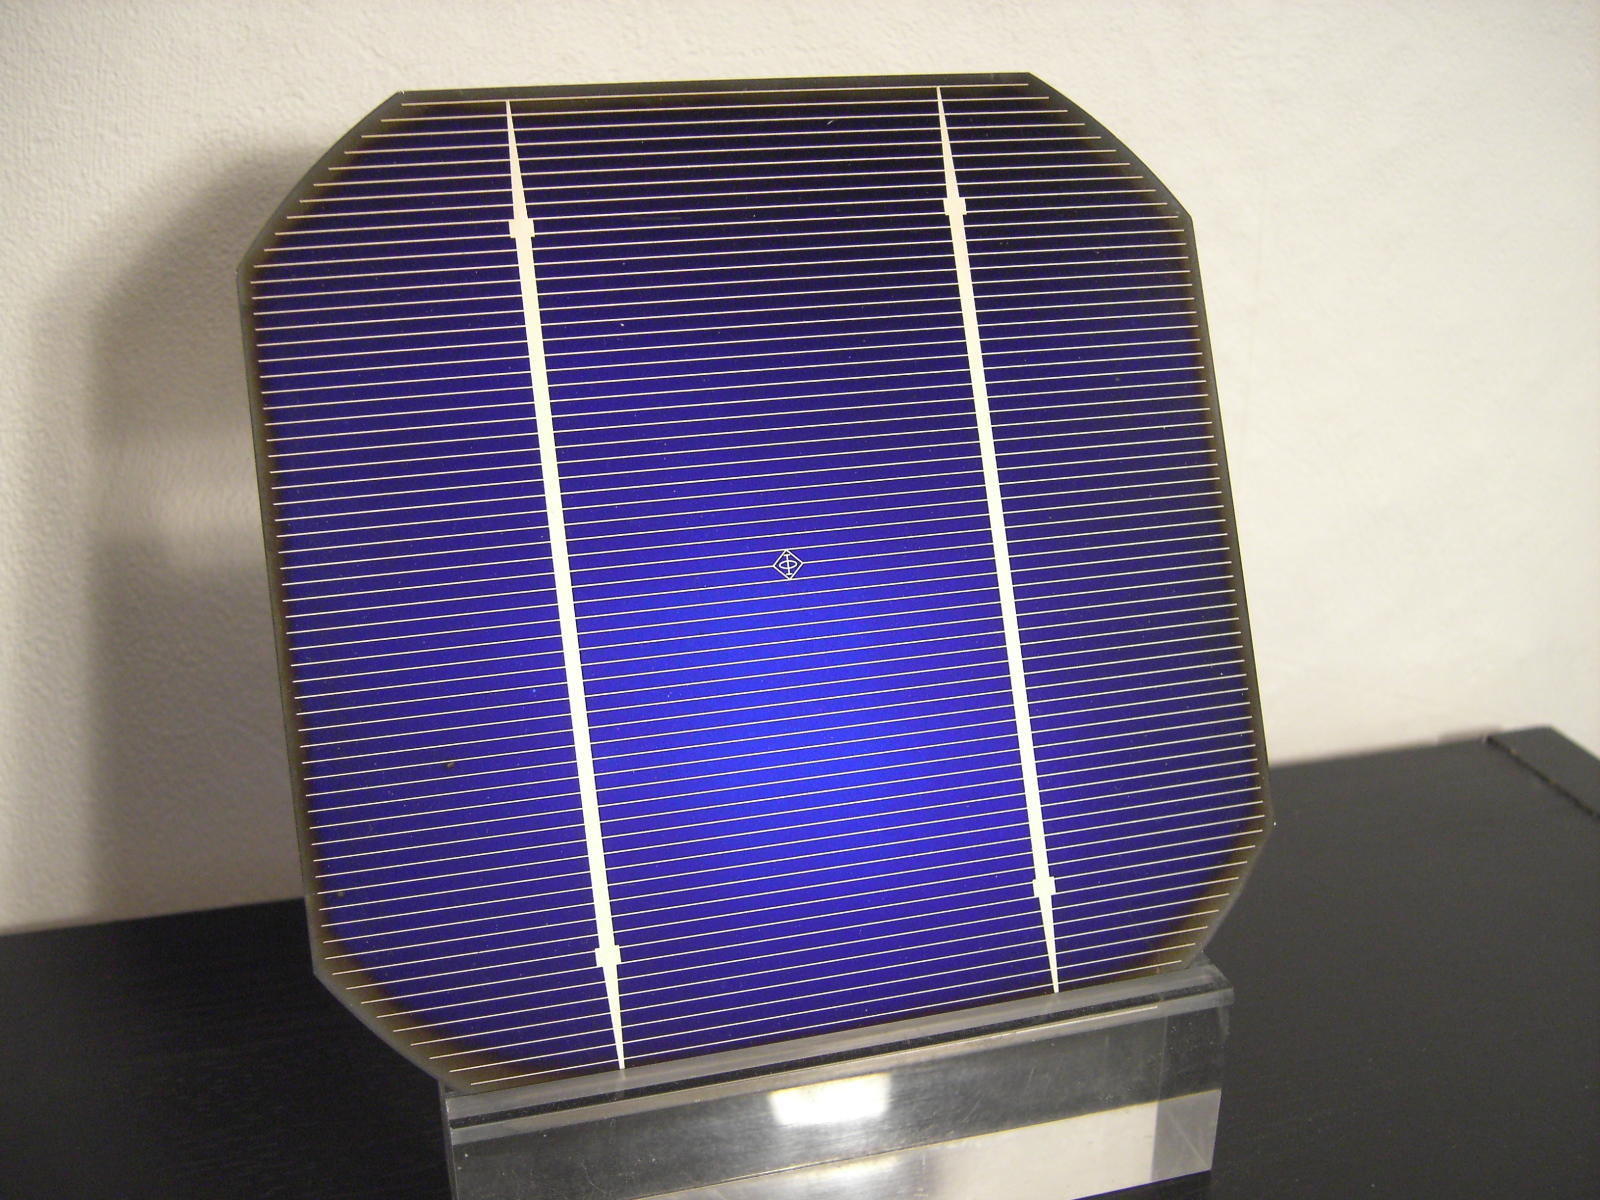
\includegraphics[width=350pt]{img/modulo-fotovoltaico.jpg}
\caption{Modulo fotovoltaico in silicio \emph{monocristallino}}
\end{figure}
%
Allo stato attuale, esistono diverse tecnologie di realizzazione di 
moduli fotovoltaici, la maggior parte delle quali basate su processi 
al silicio.
%

%
Per ogni modello di modulo fotovoltaico, le aziende 
costruttrici forniscono un \emph{datasheet}, riportanti i 
\emph{dati di targa} del modulo.
%
Tra i dati di targa, particolare importanza rivestono le curve 
\emph{corrente-tensione}, le quali caratterizzano l'andamento della tensione 
e della corrente - e, quindi, della potenza generata - ai capi del modulo, al 
variare di determinate \emph{grandezze d'influenza}.
%
Le curve corrente-tensione vengono tipicamente costruite mediante misurazioni
effettuate sotto \emph{standard test conditions} (STC)\cite{testconditions}, 
come indicato in tabella \ref{stc}, e variando di volta in volta una delle 
grandezze di influenza.
%
\begin{table}[htpb]
 \begin{center}
  \begin{tabular}{ | l | l | }
    \hline
    Radiazione & 1000 $W/m^2$ \\
    \hline
    Temperatura del modulo & 25  $\celsius$ \\
    \hline 
    Vento & 0 $m/s$ \\
    \hline
  \end{tabular}
  \caption{Condizioni di test standard (STC)}
  \label{stc}
 \end{center}
\end{table}
%

%
Un tipico esempio di curve corrente-tensione \`e mostrato in figura 
\ref{caratteristica_modulo_fv}: il primo dei due grafici mostra l'andamento 
della caratteristica al variare della radiazione solare, il secondo
invece mostra cosa accade al variare della temperatura superficiale del modulo.
%
\begin{figure}[!h]
\centering
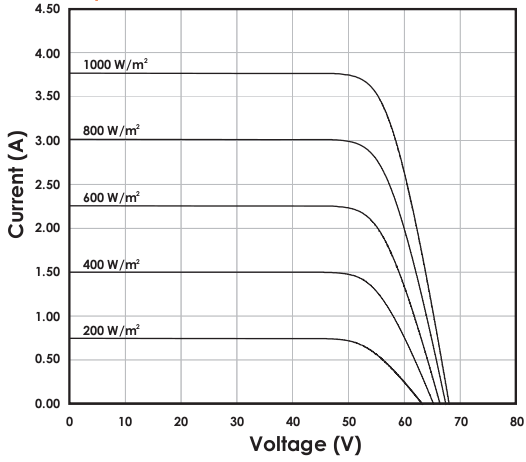
\includegraphics[width=190pt]{img/a-v-irradiance.png}
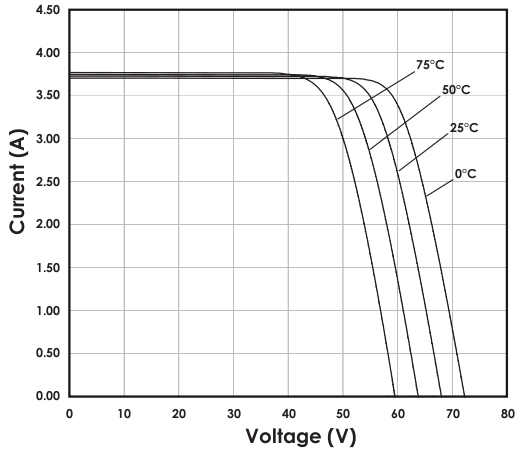
\includegraphics[width=190pt]{img/a-v-temperature.png}
\caption{Esempi di curve caratteristiche di un modulo fotovoltaico}
\label{caratteristica_modulo_fv}
\end{figure}
%% parlare della resistenza dei moduli e del decadimento delle prestazioni?
%% parlare dell'effetto dell'orientamento dei moduli rispetto alle prestazioni?
%

%
\subsection{Le stringhe fotovoltaiche}
Per \emph{stringa fotovoltaica} si intende un insieme di moduli connessi in \emph{serie}, 
come mostrato in figura \ref{stringa}.
%
La connessione in serie dei moduli \`e resa possibile da apposite \emph{junction box}, 
generalmente collocate sul retro dei moduli.
%

%
\begin{figure}[!h]
\centering
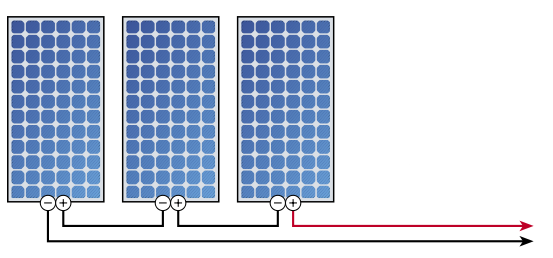
\includegraphics[width=350pt]{img/pv-string.png}
\caption{Connessione in serie di moduli fotovoltaici}
\label{stringa}
\end{figure}
%
%
\begin{figure}[!h]
\centering
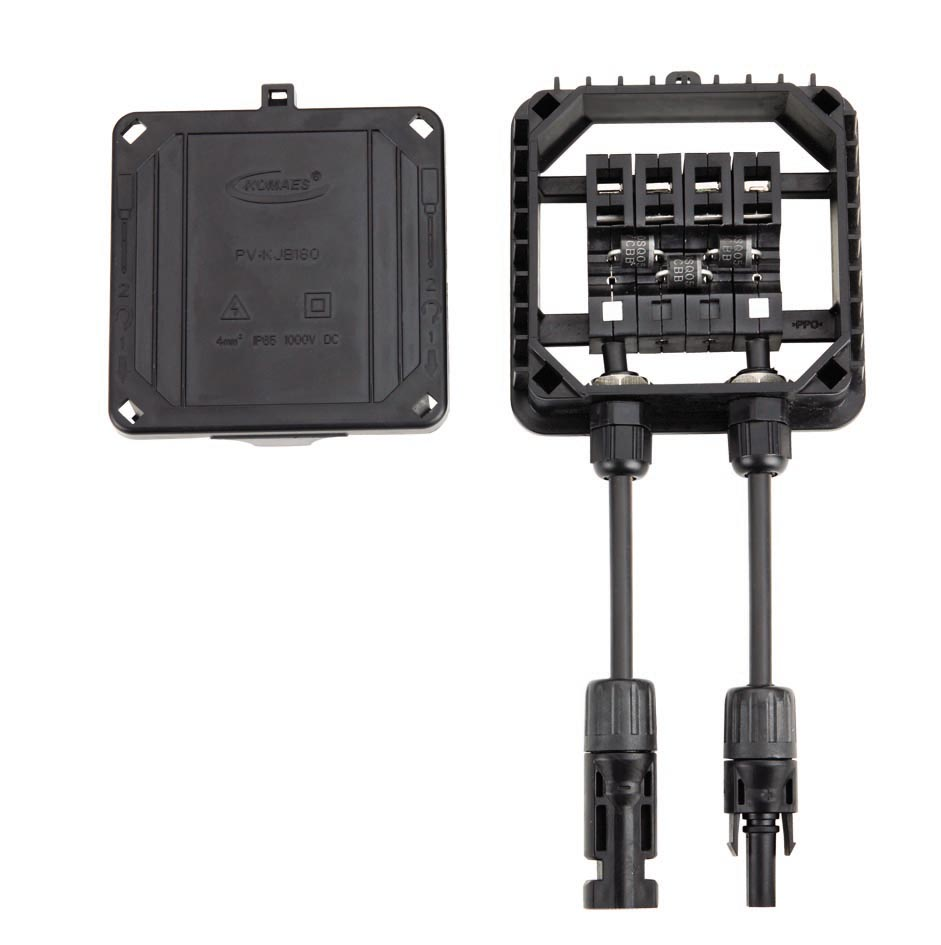
\includegraphics[width=180pt]{img/pv-junction-box.jpg}
\caption{Junction box}
\end{figure}
%

%
\`E importante evidenziare come connettere i moduli in serie condizioni le 
prestazioni dell'intera stringa: la legge di Ohm, infatti, impone che ogni 
modulo connesso in serie venga attraversato dalla stessa quantit\`a di corrente;
per cui, un degrado, anche temporaneo, delle prestazioni o, peggio, il 
malfunzionamento di uno dei moduli, provoca un peggioramento di produzione 
per tutti i moduli della stringa.
%
Tale fenomeno, noto come \emph{mismatch di corrente}, pu\`o manifestarsi,
ad esempio, nel caso in cui uno o pi\`u moduli siano, anche solo parzialmente, 
\emph{ombreggiati}, come mostrato in figura \ref{ombreggiamento}.
%
\begin{figure}[!h]
\centering
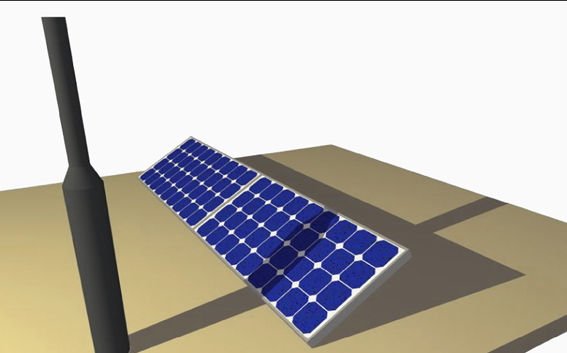
\includegraphics[width=300pt]{img/fv-ombreggiamento.png}
\caption{Ombreggiamento parziale di una stringa}
\label{ombreggiamento}
\end{figure}
%

%
Per limitare il manifestarsi di questo fenomeno, durante la fase di progettazione 
dei campi fotovoltaici vengono considerati fattori quali \Item{i} l'orientamento 
dei moduli della stringa, \Item{ii} la presenza di oggetti che possano produrre 
ombreggiamenti, \Item{iii} la distanza tra i moduli, \Item{iv} le caratteristiche 
climatiche della zona che ospiter\`a il campo fotovoltaico.
%

% dire che piu` stringhe possono essere collegate in parallelo
%
\subsection{Gli inverter}
La corrente continua prodotta dalle stringhe non pu\`o essere direttamente
immessa in rete. Si rendono necessari dei dispositivi, detti \emph{inverter}, 
in grado di trasformare la corrente continua in corrente alternata, alla 
stessa frequenza di quella della rete di distribuzione.
%

%
Nel contesto di un campo fotovoltaico, gli inverter sono quindi collocati a 
giunzione delle stringhe con la rete di distribuzione esterna. 
%
Come intuibile, si tratta dei componenti pi\`u complessi e critici degli 
impianti fotovoltaici: una loro avaria pu\`o compromettere il processo di 
distribuzione dell'energia prodotta dai moduli.
%

%
%
\begin{figure}[!h]
\centering
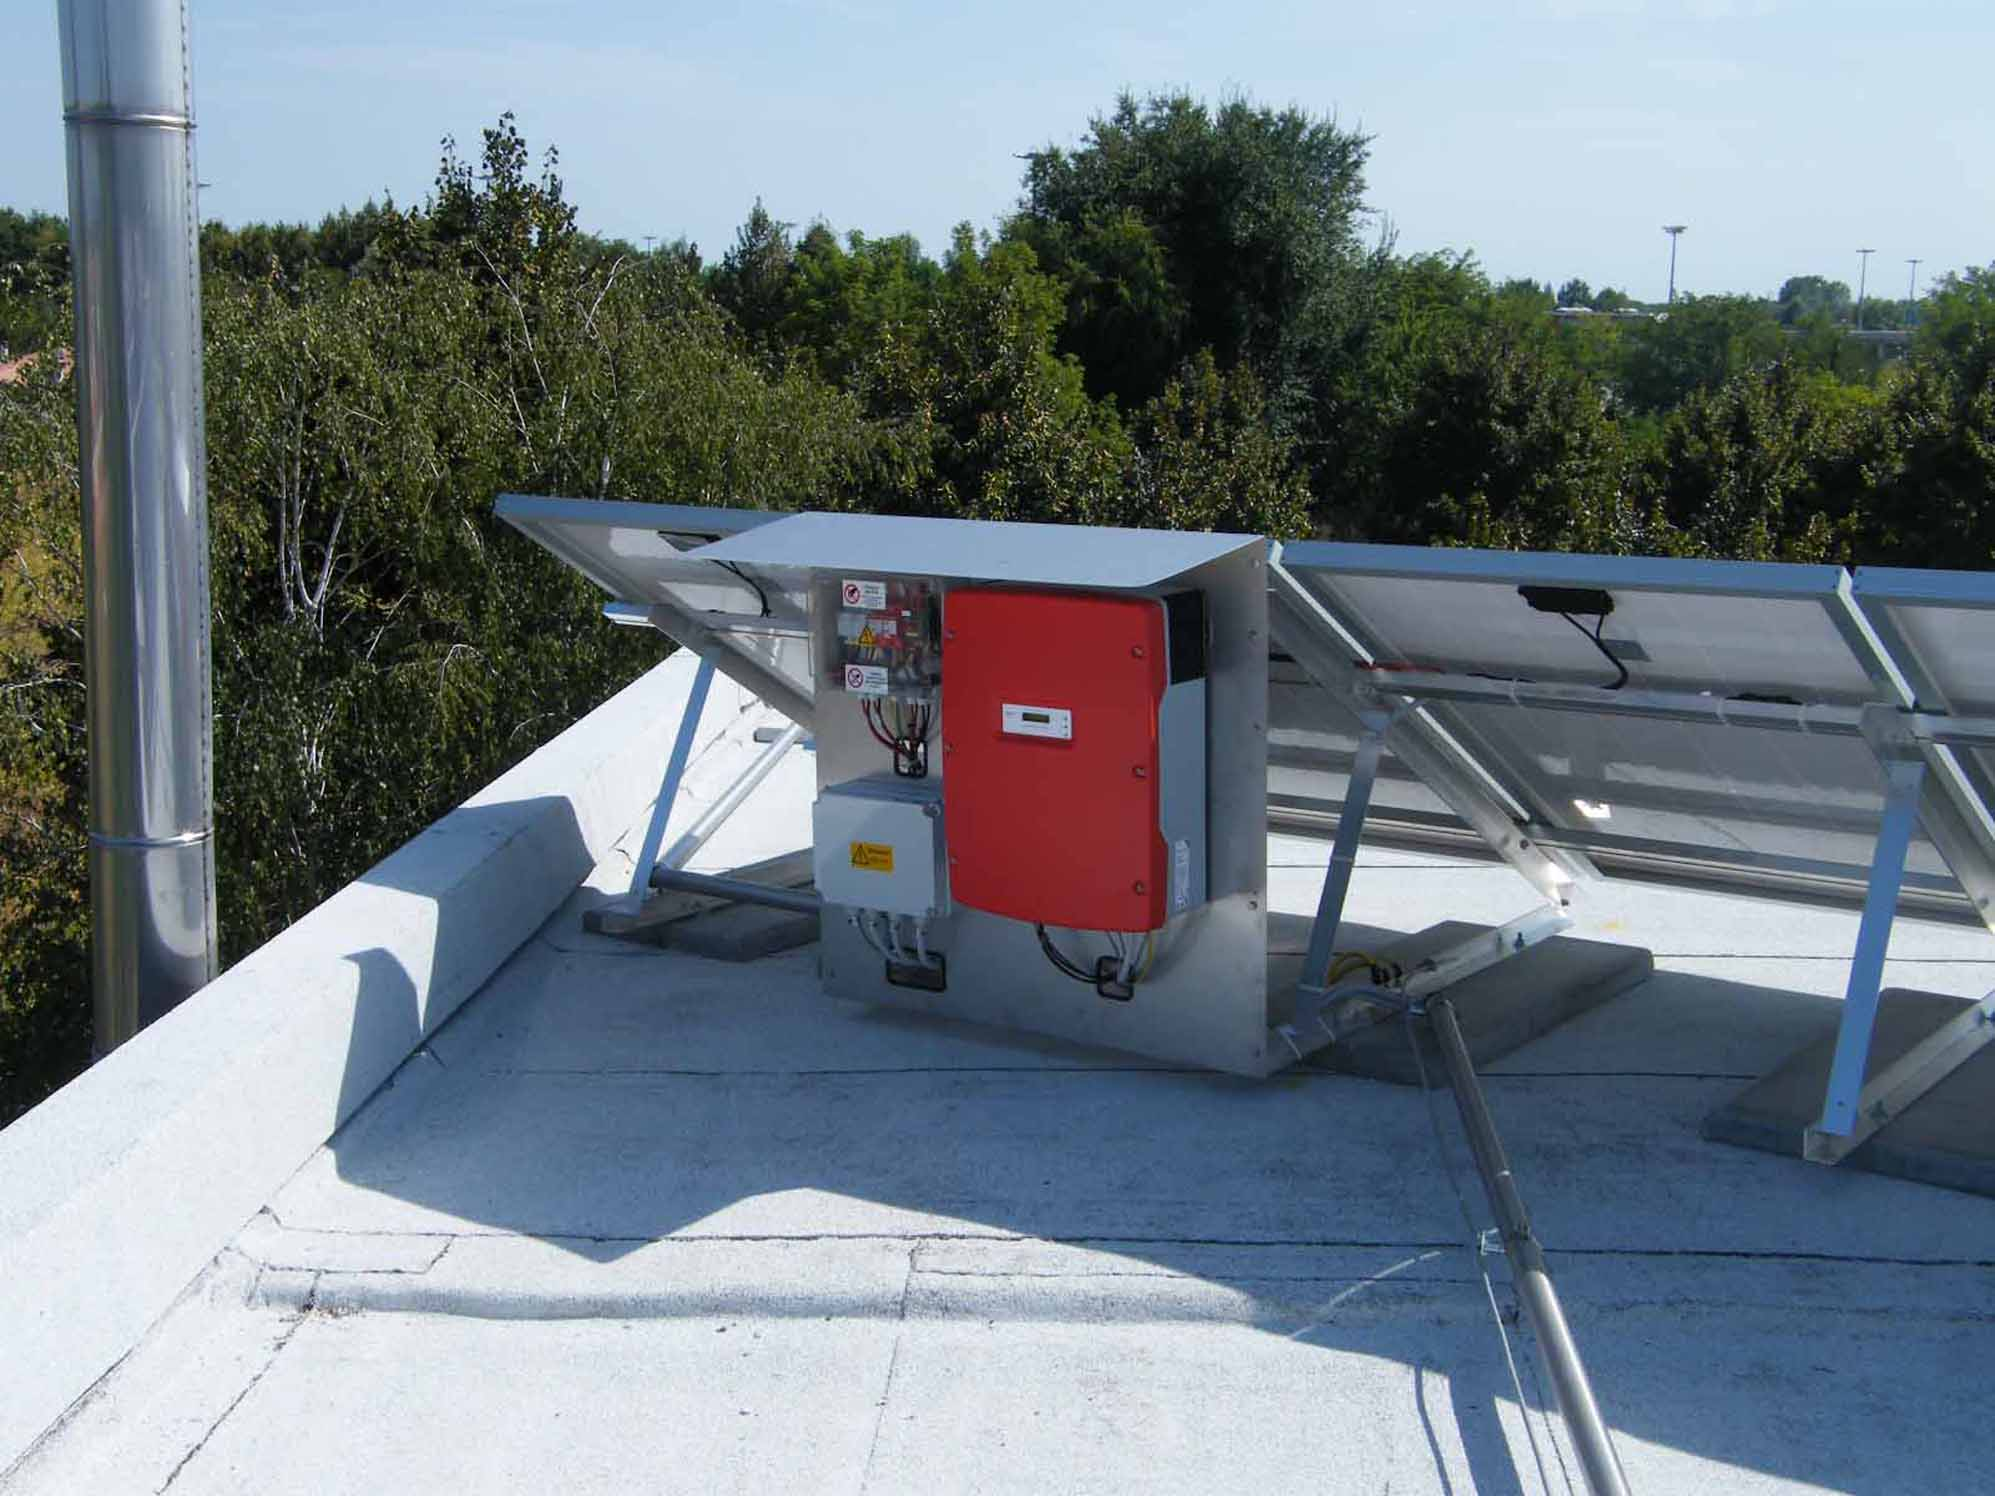
\includegraphics[width=300pt]{img/pv-inverter.jpg}
\caption{Inverter fotovoltaico}
%%\label{ombreggiamento}
\end{figure}
%
Tra i dati di targa di un inverter, particolare importanza riveste la sua 
\emph{efficienza}, definita come il rapporto tra l'energia in uscita 
(ceduta dall'inverter alla rete di distribuzione) e l'energia in ingresso 
(prodotta dalle stringhe).
%
Il valore di efficienza di un inveter non \`e determinato solo dalla 
non idealit\`a del processo di trasfomazione: parte dell'energia in ingresso, 
infatti, viene utilizzata dallo stesso inverter come alimentazione.
%
Gli inverter oggi presenti in commercio sono caratterizzati da valori tipici di
efficienza superiori al 95\%. Tuttavia, \`e da tenere in conto che l'efficienza 
di un inverter, a causa dell'effetto combinato di tempo e usura, tende a 
subire delle degradazioni.
%

%
Gli inverter progettati specificatamente per il fovoltaico presentano una gamma 
di funzionalit\`a che va oltre la sola trasformazione di corrente continua 
in alternata. Essi, infatti, sono spesso dotati di particolari sistemi di 
controllo, come il \emph{maximum power point tracker} (MPPT) che regolano la tensione 
di stringa in modo tale da estrarre dai moduli la massima potenza disponibile 
in qualsiasi condizione di irraggiamento.
%

%
Opzionalmente, gli inverter possono anche essere provvisti di un \emph{data logger}, 
i.e. un dispositivo che registra, nel tempo, i valori di grandezze di interesse quali 
correnti, tensioni, potenze ed energia prodotta.
% di notte gli inverter si spengono

%
\subsection{Il problema del rifasamento}
%
In regime di corrente alternata, la potenza elettrica $(S)$ \`e il risultato della 
somma di due componenti vettoriali: una \emph{attiva} $(P)$, traformabile in 
\emph{lavoro} e una \emph{reattiva} $(Q)$.
%
La presenza della componente reattiva \`e il diretto risultato dell'azione delle 
reattanze presenti in un circuito, i.e. induttori e/o condensatori, le quali 
provocano uno \emph{sfasamento} tra corrente e tensione, rappresentato in 
figura \ref{potenzaattivareattiva} dall'angolo $\varphi$.
%

%
\begin{figure}[!h]
\centering
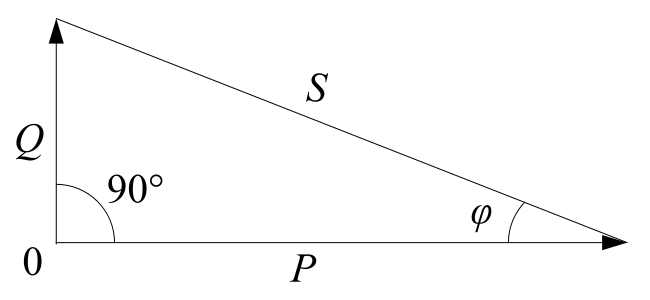
\includegraphics[width=250pt]{img/apparent-power.png}
\caption{Rappresentazione vettoriale di potenza attiva e reattiva}
\label{potenzaattivareattiva}
\end{figure}
%
Bench\'e si tratti di una componente inutilizzabile, la presenza della potenza 
reattiva va tenuta in considerazione nel dimensionamento dei sistemi di 
distribuzione. \`E per questo motivo che il gestore della rete elettrica in 
bassa tensione impone dei limiti circa le quantit\`a di potenza reattiva 
che le utenze sono autorizzate a scambiare con la rete stessa.
%

%
Per rispettare tali limiti, indicati in \cite{criteriallacciamento}, gli impianti 
fotovoltaici possono essere dotati di sistemi di \emph{rifasamento}, posti 
tra gli inverter e il contatore di scambio, il cui scopo \`e l'azzeramento 
dell'angolo $\varphi$.
%

%
\section{Il problema del monitoraggio}
Terminata la breve panoramica sugli impianti fotovoltaici, introduciamo il 
problema alla base del presente lavoro di tesi: il monitoraggio degli impianti 
fotovoltaici.
%

%
Il problema del monitoraggio pu\`o essere formulato mutuando concetti e 
terminologia dalla disciplina del \emph{controllo dei processi industriali}: 
la produzione di energia elettrica mediante moduli fotovoltaici pu\`o essere
modellata, infatti, come un \emph{processo continuo} caratterizzato dalle 
seguenti \emph{variabili di stato}:
%
\begin{itemize}

\end{itemize}



%% cosa monitorare: tensioni, correnti, potenze, energie
%% cosa monitorare: degradazione delle performance dei singoli componenti





%% architettura tipica di un impianto fotovoltaico
%% quali informazioni si vogliono produrre?
%% quali informazioni e` necessario rilevare?
%% lista dei desiderata per un sistema di monitoraggio
